\chapter{Custionario a alumnos}
\label{Appendix:cuestionarios}

\textbf{¿En qué punto de tu carrera te encuentras actualmente?}
\begin{figure}[H]
	\centering
	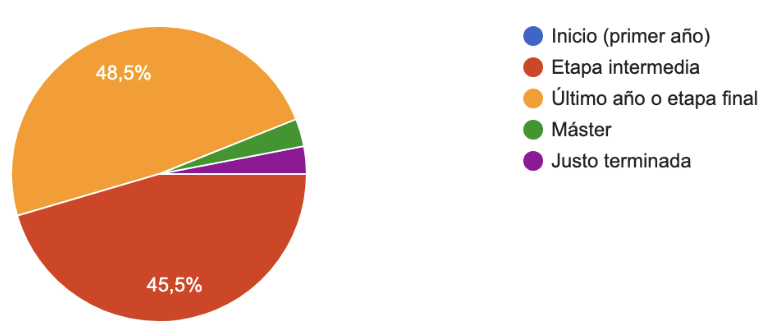
\includegraphics[width = 0.6\textwidth]{Imagenes/Respuestas_Cuestionarios/r1.png}
	\caption{Distribución de los encuestados según su etapa académica actual}
	\label{fig:año}
\end{figure}

\textbf{¿Qué estudias?}
\begin{figure}[H]
	\centering
	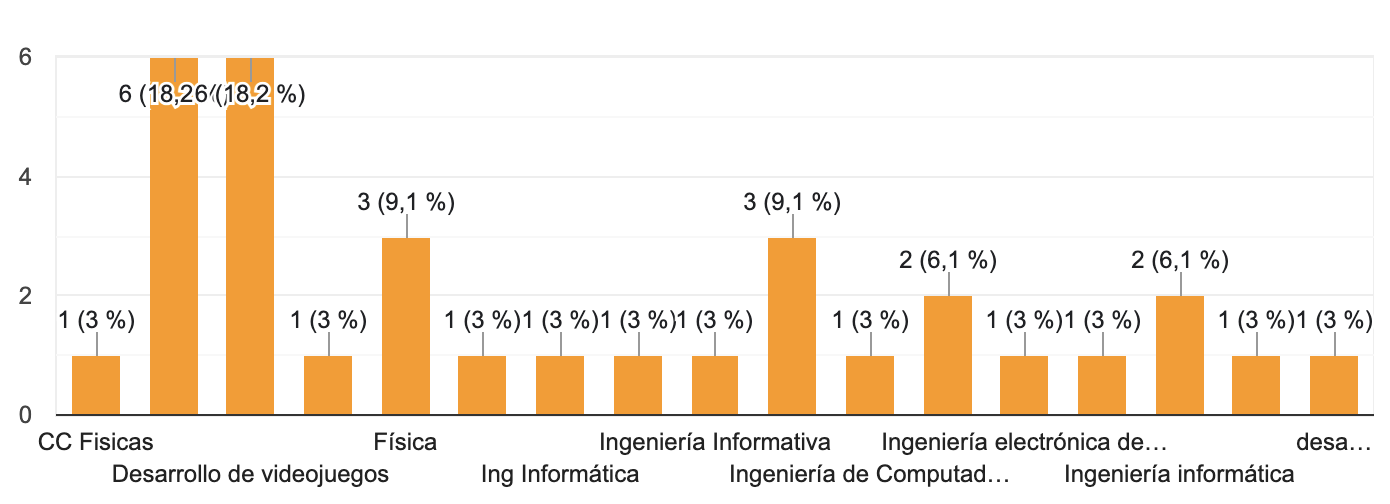
\includegraphics[width = 0.6\textwidth]{Imagenes/Respuestas_Cuestionarios/r2.png}
	\caption{Diversidad de carreras}
	\label{fig:estudios}
\end{figure}


\textbf{En la siguiente escala, ¿cómo de difícil es para ti entender el enunciado a la hora de afrontar el ejercicio?}
\begin{figure}[H]
	\centering
	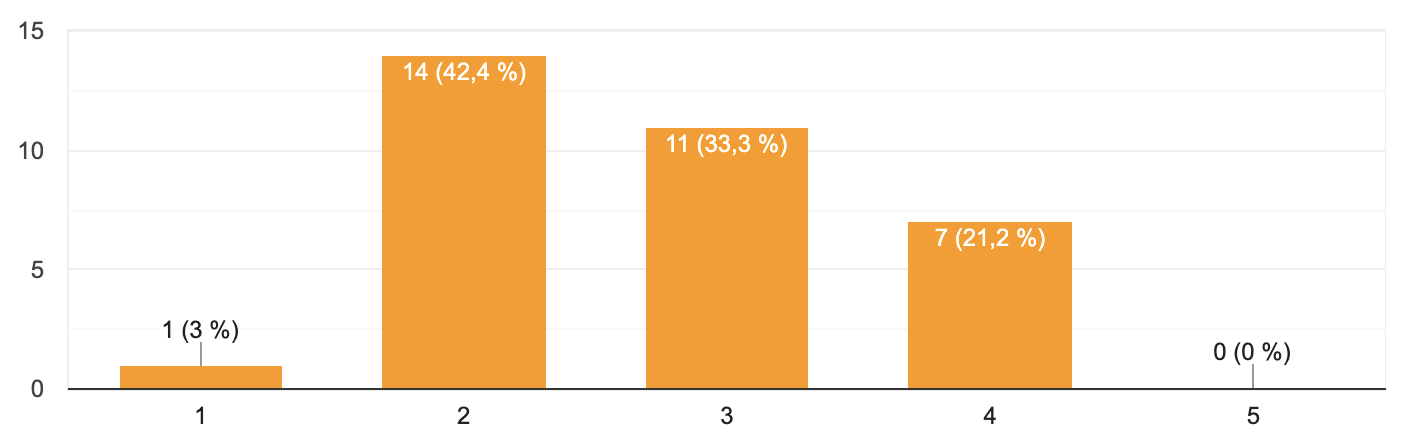
\includegraphics[width = 0.6\textwidth]{Imagenes/Respuestas_Cuestionarios/r3.png}
	\caption{Dificultad percibida en la comprensión del enunciado.}
	\label{fig:entender_enunciado}
\end{figure}

\textbf{En la siguiente escala, ¿cómo de difícil es para ti pensar el algoritmo a la hora de afrontar el ejercicio?}
\begin{figure}[H]
	\centering
	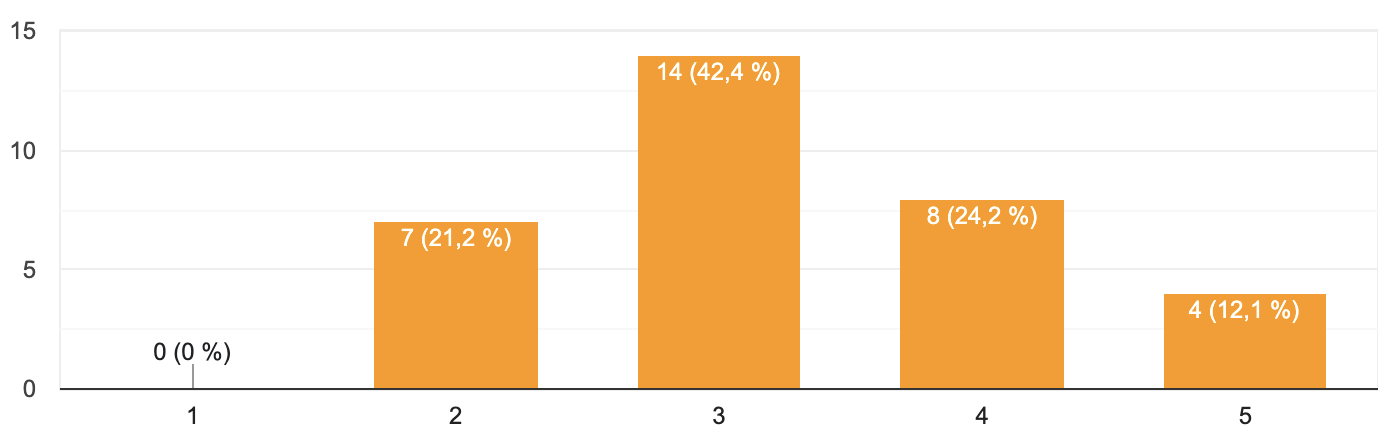
\includegraphics[width = 0.6\textwidth]{Imagenes/Respuestas_Cuestionarios/r4.png}
	\caption{Gráfica dificultad pensar algoritmo}
	\label{fig:pensar_algoritmo}
\end{figure}

\textbf{En la siguiente escala, ¿cómo de difícil es para ti detectar errores en tu solución a la hora de resolver un ejercicio?}
\begin{figure}[H]
	\centering
	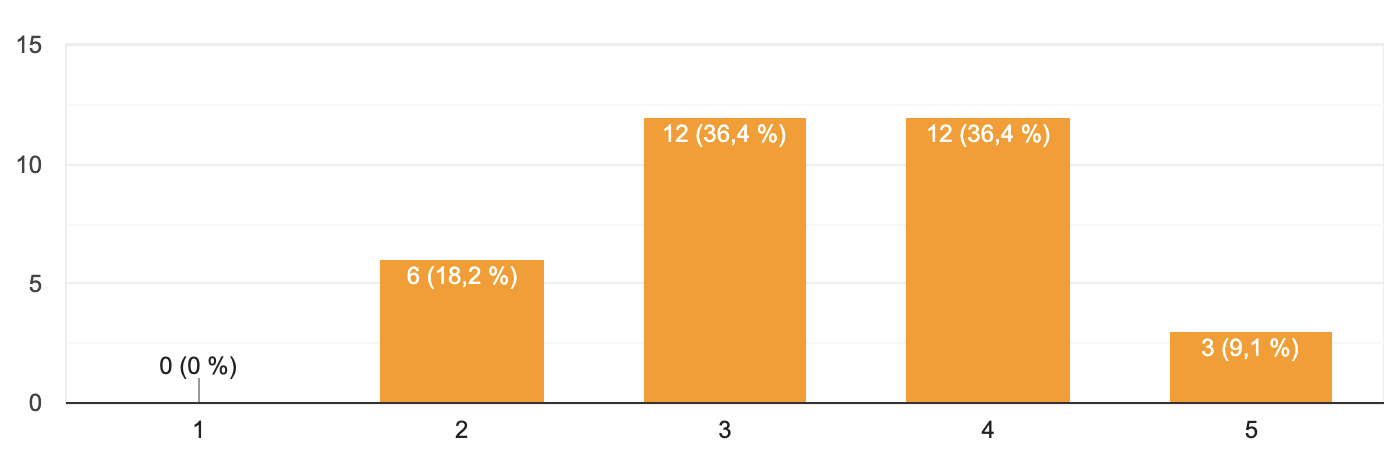
\includegraphics[width = 0.6\textwidth]{Imagenes/Respuestas_Cuestionarios/r5.png}
	\caption{Nivel de dificultad reportado al diseñar algoritmos}
	\label{fig:detectar_errores}
\end{figure}

\textbf{En la siguiente escala, ¿cómo de difícil es para ti encontrar contraejemplos para probar tu código a la hora de resolver un ejercicio?}
\begin{figure}[H]
	\centering
	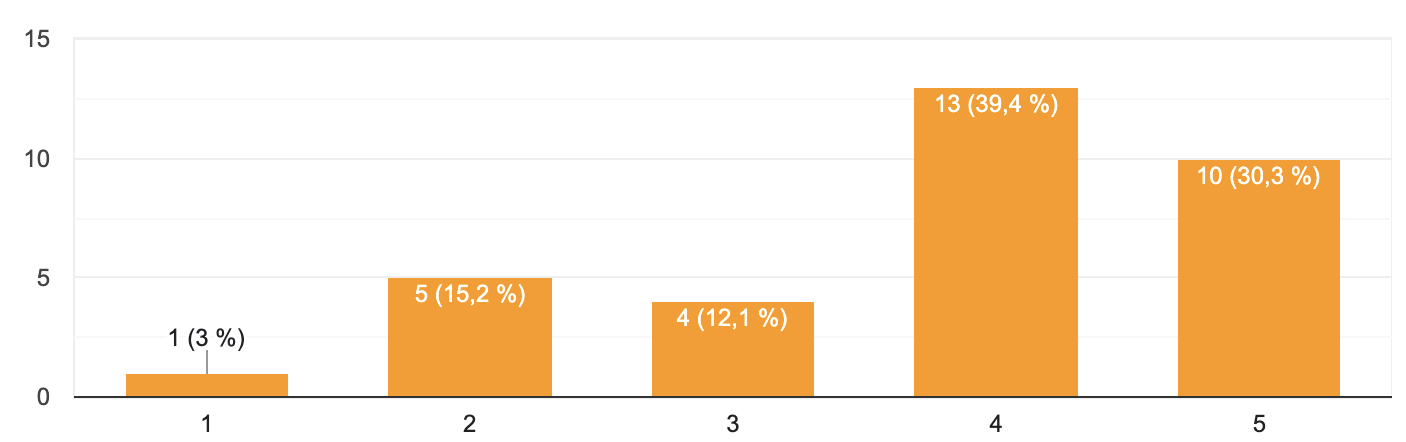
\includegraphics[width = 0.6\textwidth]{Imagenes/Respuestas_Cuestionarios/r6.png}
	\caption{Dificultad encontrar contraejemplos}
	\label{fig:encontrar_contraejemplos}
\end{figure}

\textbf{En la siguiente escala, ¿cuánto afecta a tu estudio saber si tu solución es correcta a la hora de entregar un ejercicio?}
\begin{figure}[H]
	\centering
	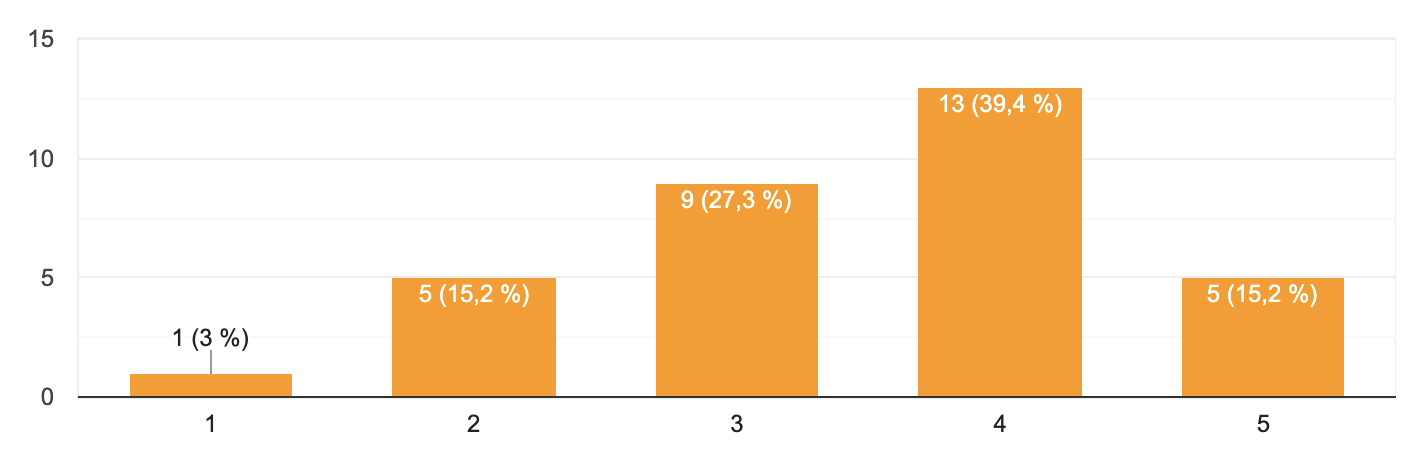
\includegraphics[width = 0.6\textwidth]{Imagenes/Respuestas_Cuestionarios/r7.png}
	\caption{Impacto conocer la solución correcta}
	\label{fig:solución_correcta}
\end{figure}

\textbf{En la siguiente escala, ¿cuánto te afecta no recibir un feedback claro sobre tu solución a la hora de entregar un ejercicio?}
\begin{figure}[H]
	\centering
	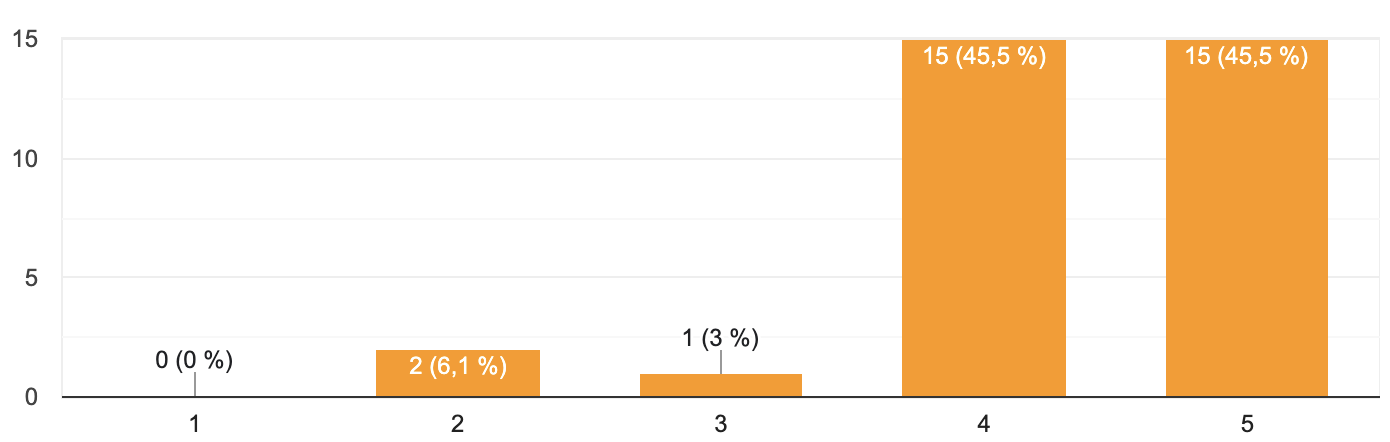
\includegraphics[width = 0.6\textwidth]{Imagenes/Respuestas_Cuestionarios/r8.png}
	\caption{Impacto del feedback recibido}
	\label{fig:impacto_feedback}
\end{figure}

\textbf{¿Qué haces normalmente cuando tu código no funciona? (Selecciona todas las que necesites)}
\begin{itemize}
    \item Pruebo casos simples
    \item Lo busco en internet o consulto con alguna herramienta de IA
    \item Escribo al profesor
    \item Pido ayuda a un compañero
    \item Lo empiezo de 0
    \item Reviso cada línea de código
    \item Uso prints para ver la información que se va guardando
    \item Uso el depurador del IDE
    \item Lo abandono
    \item Otro:
\end{itemize}
\begin{figure}[H]
	\centering
	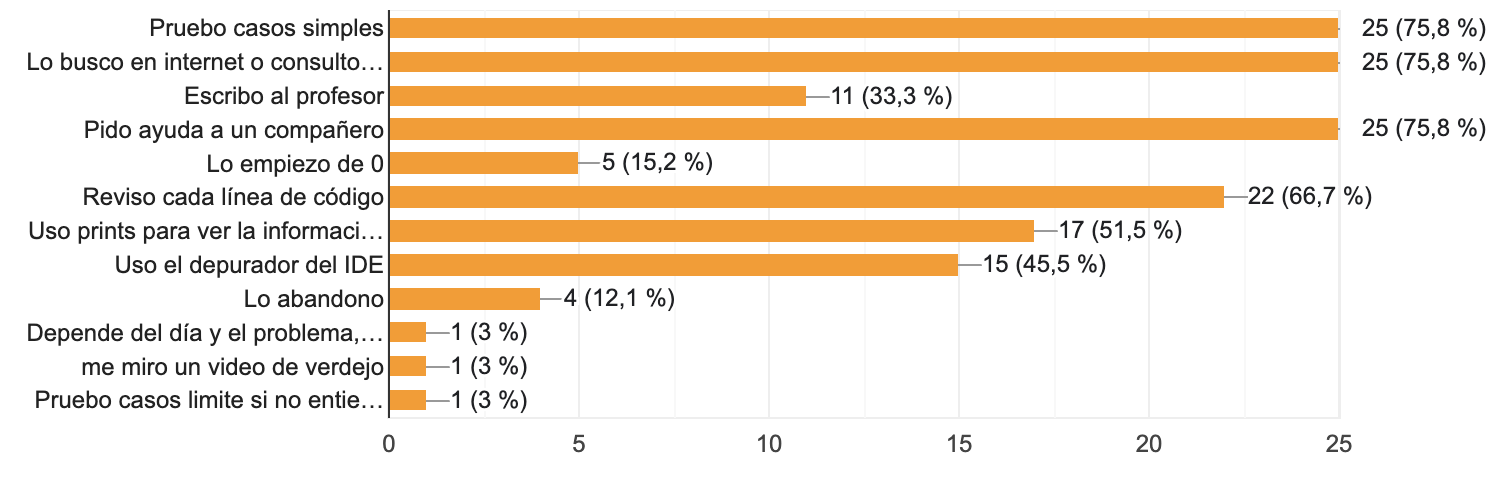
\includegraphics[width = 0.7\textwidth]{Imagenes/Respuestas_Cuestionarios/r9.png}
	\caption{Comportamiento cuando el código no funciona}
	\label{fig:comportamiento_código_erróneo}
\end{figure}

\textbf{Cuando debuggeas un código, ¿qué información te gusta ver? (Selección múltiple)}
\begin{itemize}
    \item Valor de las variables
    \item Mensaje y línea de error
    \item Comparación entre mi salida y la esperada
    \item Casos de prueba que fallan
    \item No me fijo en nada específico, solo cuándo falla
    \item Otro:
\end{itemize}
\begin{figure}[H]
	\centering
	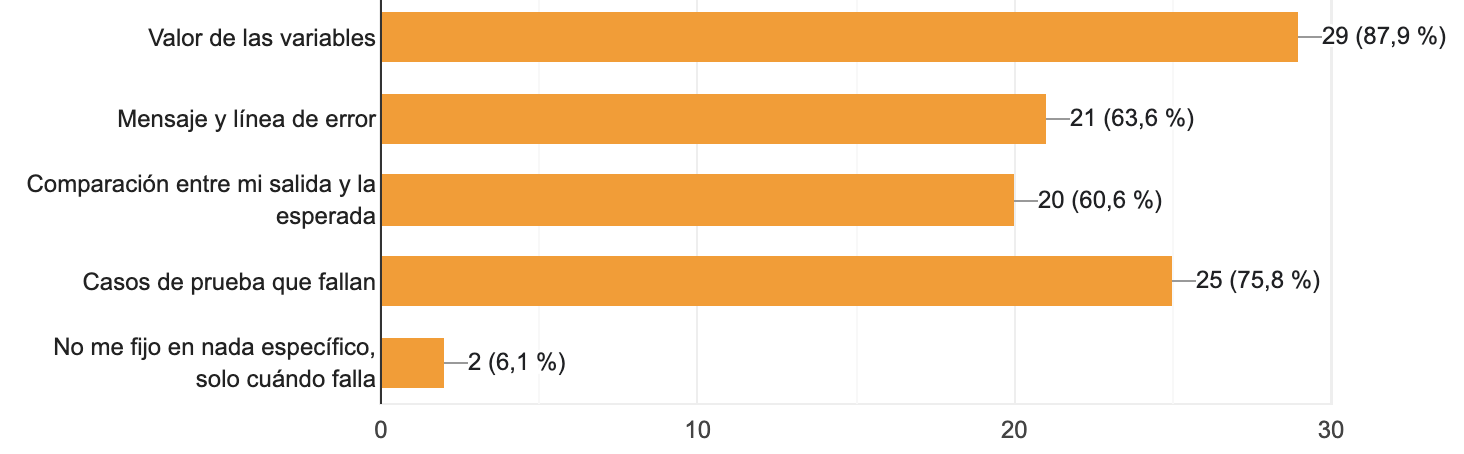
\includegraphics[width = 0.7\textwidth]{Imagenes/Respuestas_Cuestionarios/r10.png}
	\caption{Información considerada como útil al debuggear}
	\label{fig:info_debug}
\end{figure}

\textbf{En la siguiente escala, ¿cómo de útil te resultaría un feedback que te muestre dónde falla tu código?}
\begin{figure}[H]
	\centering
	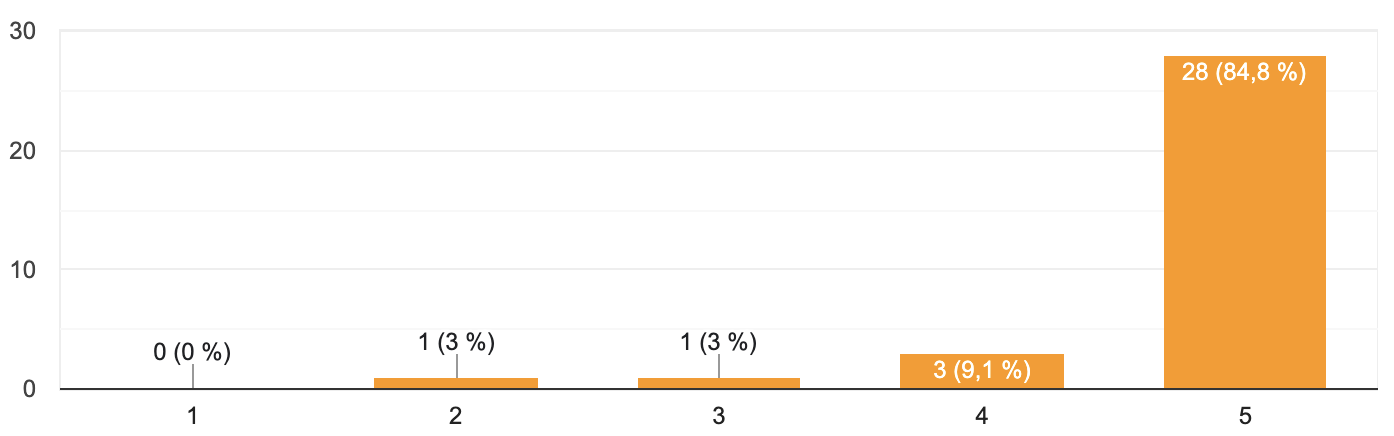
\includegraphics[width = 0.6\textwidth]{Imagenes/Respuestas_Cuestionarios/r11.png}
	\caption{Opinión posible feedback que muestre dónde falla}
	\label{fig:feedback_fallo}
\end{figure}

\textbf{En la siguiente escala, ¿cómo de útil te resultaría un feedback que te proporcione un contrajemplo que falla en tu código?}
\begin{figure}[H]
	\centering
	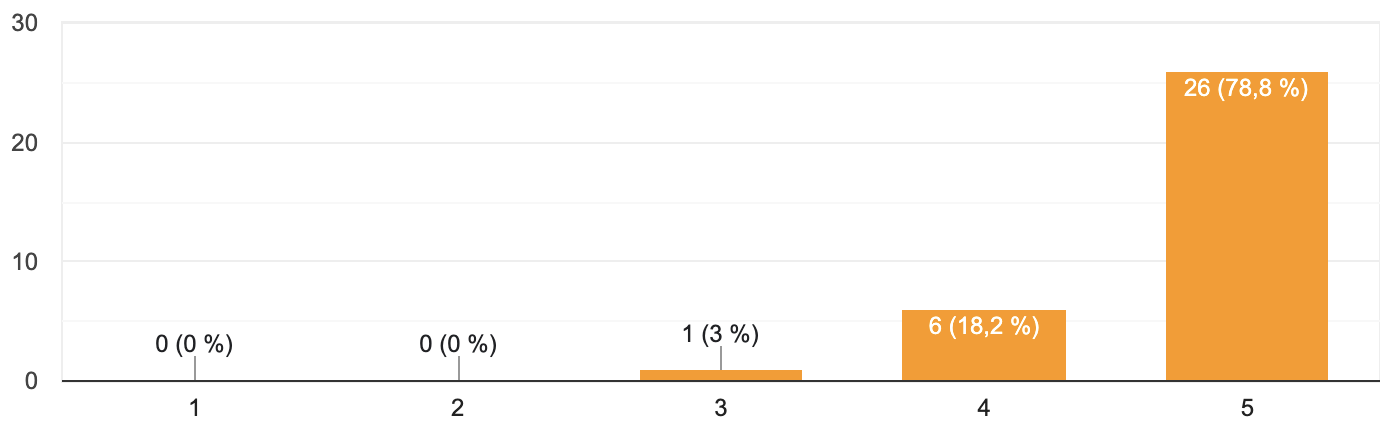
\includegraphics[width = 0.6\textwidth]{Imagenes/Respuestas_Cuestionarios/r12.png}
	\caption{Opinión posible feedback con contraejemplo}
	\label{fig:feedback_contraejemplo}
\end{figure}

\textbf{En la siguiente escala, ¿cómo de útil te resultaría un feedback con una explicación teórica?}
\begin{figure}[H]
	\centering
	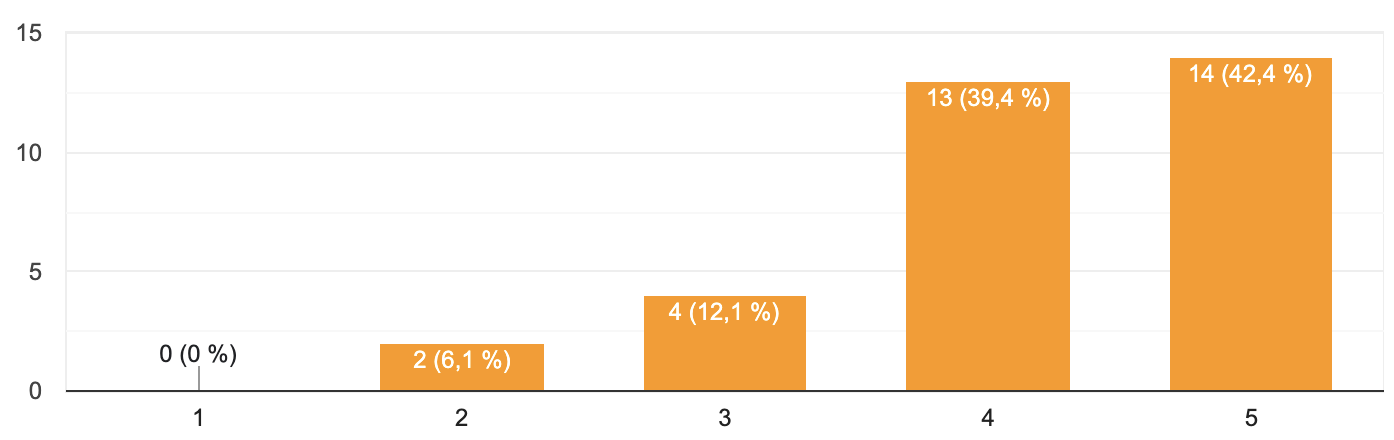
\includegraphics[width = 0.6\textwidth]{Imagenes/Respuestas_Cuestionarios/r13.png}
	\caption{Opinión posible feedback con explicación teórica}
	\label{fig:feedback_explicación_teórica}
\end{figure}

\textbf{En la siguiente escala, ¿cómo de útil te resultaría un feedback que compare tu salida con la salida esperada?}
\begin{figure}[H]
	\centering
	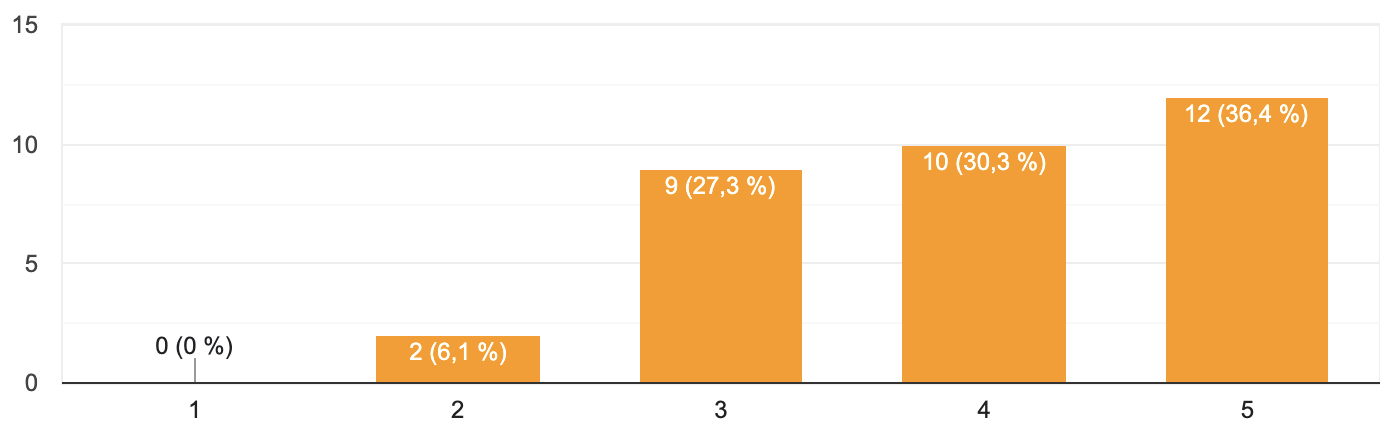
\includegraphics[width = 0.6\textwidth]{Imagenes/Respuestas_Cuestionarios/r14.png}
	\caption{Opinión posible feedback con comparación de salidas}
	\label{fig:feedback_comparación_salidas}
\end{figure}

\textbf{En la siguiente escala, ¿cómo de útil te resultaría un feedback que te de una pista sobre el error que hay en tu código?}
\begin{figure}[H]
	\centering
	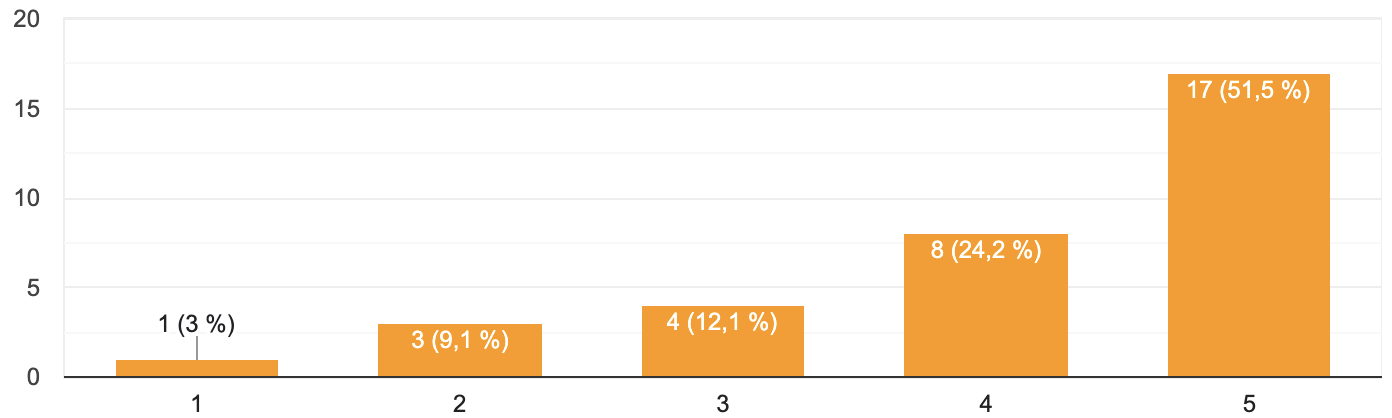
\includegraphics[width = 0.6\textwidth]{Imagenes/Respuestas_Cuestionarios/r15.png}
	\caption{Opinión posible feedback con pistas sobre el error}
	\label{fig:feedback_pistas}
\end{figure}

\textbf{En la siguiente escala, ¿cómo de útil te resultaría un feedback que te visualice por qué está bien o mal tu código?}
\begin{figure}[H]
	\centering
	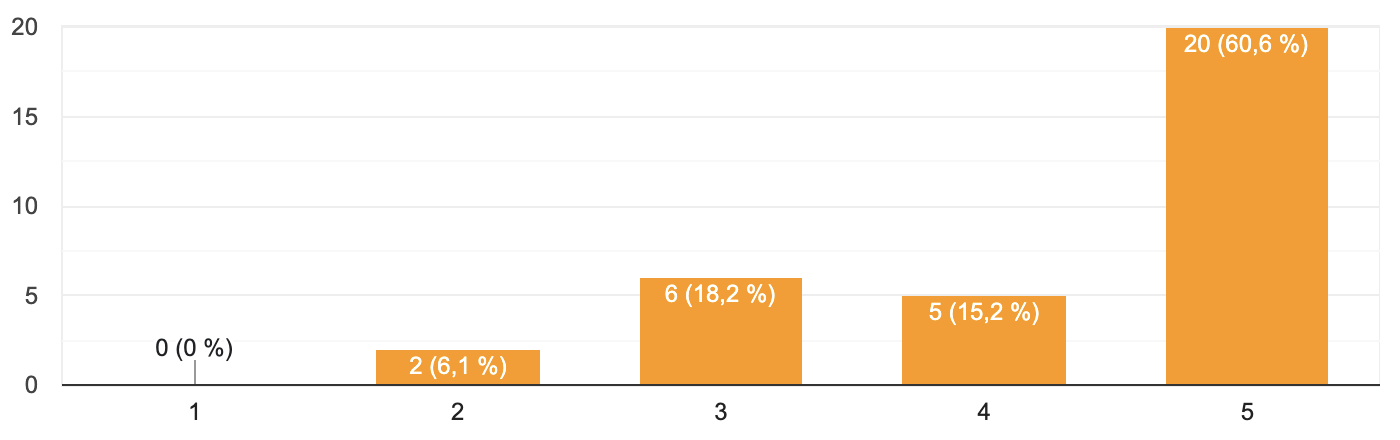
\includegraphics[width = 0.6\textwidth]{Imagenes/Respuestas_Cuestionarios/r16.png}
	\caption{Opinión posible feedback con visualización}
	\label{fig:feedback_visualización}
\end{figure}

\textbf{¿Sueles dibujar estructuras (listas, pilas, árboles, diagramas, etc.) para entender o resolver un ejercicio de estructuras de datos?}
\begin{figure}[H]
	\centering
	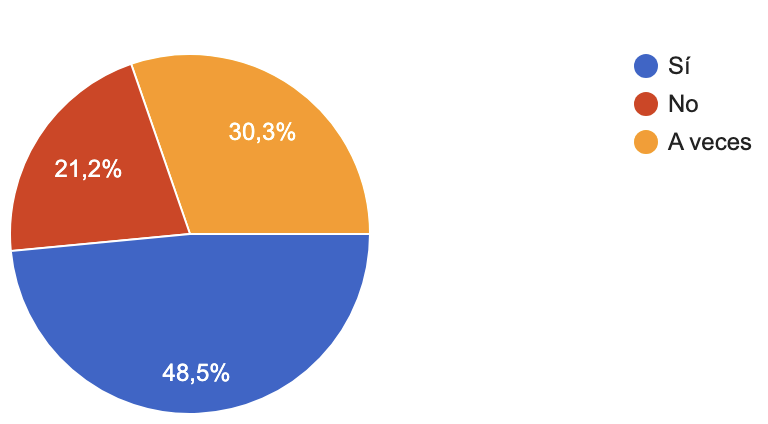
\includegraphics[width = 0.6\textwidth]{Imagenes/Respuestas_Cuestionarios/r17.png}
	\caption{Frecuencia representación estructuras}
	\label{fig:dibujo_estructuras}
\end{figure}

\textbf{¿Qué herramientas has usado más para practicar ejercicios de programación?}
\begin{itemize}
    \item DOMjudge
    \item HackerRank
    \item LeetCode
    \item Moodle
    \item Codeforces
    \item Acepta el reto
    \item Ninguna
    \item Otro:
\end{itemize}
\begin{figure}[H]
	\centering
	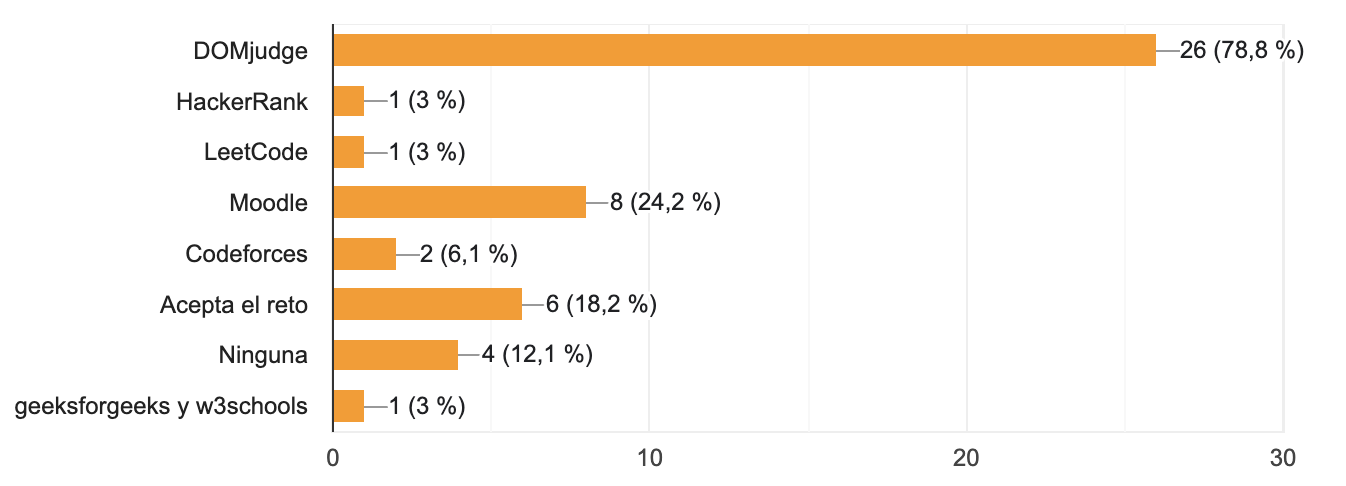
\includegraphics[width = 0.7\textwidth]{Imagenes/Respuestas_Cuestionarios/r18.png}
	\caption{Herramientas más utilizadas para resolución de ejercicios de programación}
	\label{fig:herramientas_mas_usadas}
\end{figure}

\textbf{¿Qué características te gustan más de esas plataformas? (Selección múltiple)}
\begin{itemize}
    \item Corrección automática inmediata.
    \item Ver si el ejercicio está bien o mal al instante.
    \item Disponibilidad de casos de prueba.
    \item Explicaciones o \textit{hints}.
    \item Interfaz clara y fácil de usar.
    \item Ejemplos de ejecución.
    \item Estadísticas o progreso.
    \item Gamificación (puntos, rankings…).
    \item Poder comparar con soluciones de otros.
    \item No sabría decir.
    \item Otro.
\end{itemize}
\begin{figure}[H]
	\centering
	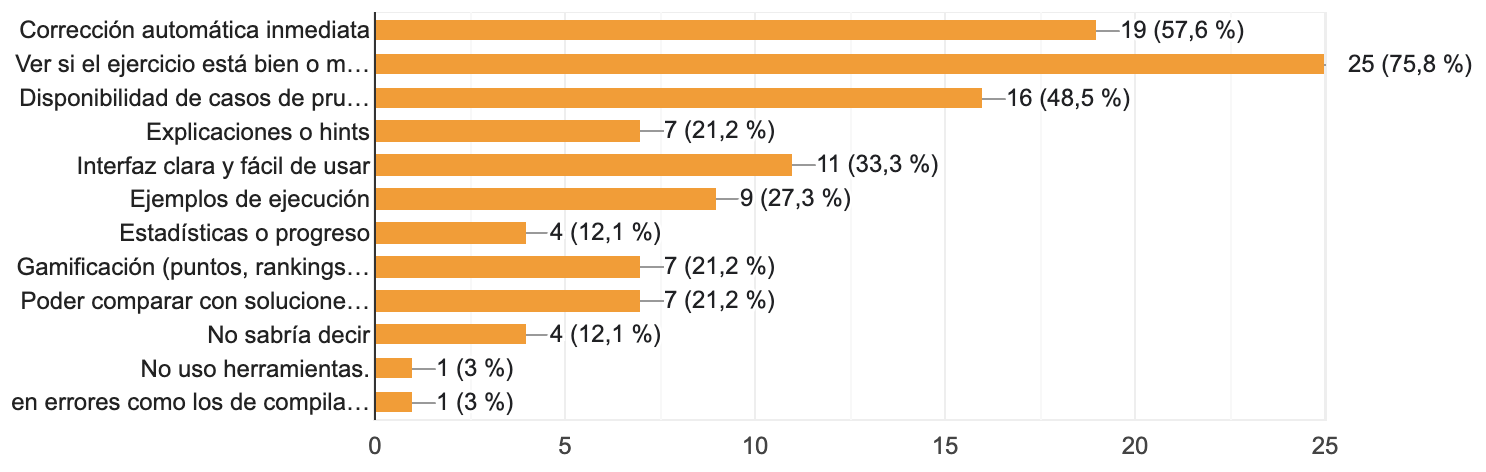
\includegraphics[width = 0.7\textwidth]{Imagenes/Respuestas_Cuestionarios/r20.png}
	\caption{Características más valoradas de las herramientas}
	\label{fig:características_herramientas}
\end{figure}

\textbf{¿Qué cosas mejorarías de las herramientas actuales que usas? (Respuesta libre)}

A continuación se transcriben las respuestas literales de los alumnos:
\begin{itemize}
    \item Pues de DOMJudge mejoraría que te explique el caso de uso en el que ha fallado y la diferencia de tu resultado con el correcto.
    \item Más información sobre los errores.
    \item Más ejemplos y contraejemplos.
    \item Que me digan qué falla o me den más casos de prueba o el caso exacto en el que falla.
    \item Mejorar el feedback.
    \item Más explicaciones de por qué está mal.
    \item Ejemplos de cómo se resuelve correctamente el ejercicio.
    \item Que no sean tan exquisitas a errores de escritura como escribir “si” en vez de “Si”.
    \item Que al fallar un caso te diga el que ha fallado o algo por el estilo. Supongo que así te puede acabar dando todos los casos, pero tener que preguntarle al profesor cada vez es incómodo.
    \item Que entre en más detalle a la hora de encontrar un error.
    \item Ejemplos que suelan dar fallo o alguna pista relacionada con por qué está mal mi código específicamente.
    \item Que te den la opción de enviarte qué input no te da bien al momento.
    \item Feedback de los errores, saber en qué punto salta el error. Más casos de prueba, especialmente casos límite.
    \item Que cuando me dice WRONG-ANSWER me diga cuál está mal.
    \item Los jueces son demasiado estrictos; mi respuesta puede estar bien, pero porque no lo he hecho en el formato adecuado me da mal. DOMJudge no te dice dónde o por qué has fallado.
    \item Que te muestre los casos en los que da error y cuáles son los valores que ha introducido en esos casos.
    \item Simplemente que me diga en qué caso falla y así no tener que pedirselo al profesor.
    \item Que me dieran acceso al código de otros que les sale bien para ver en qué fallo, o un asistente que me indique cómo mejorar mi código.
    \item Que el programa proporcionara con cada subida errónea una serie de casos que hacen que tu código falle.
    \item El problema principal está en que cuesta mucho encontrar el contraejemplo donde falla. Estaría muy bien que la plataforma me facilitara el caso en el que mi código no funciona para no volverme loca buscándolo.
\end{itemize}

\textbf{¿Utilizas casos de prueba para probar tus soluciones?}
\begin{figure}[H]
    \centering
    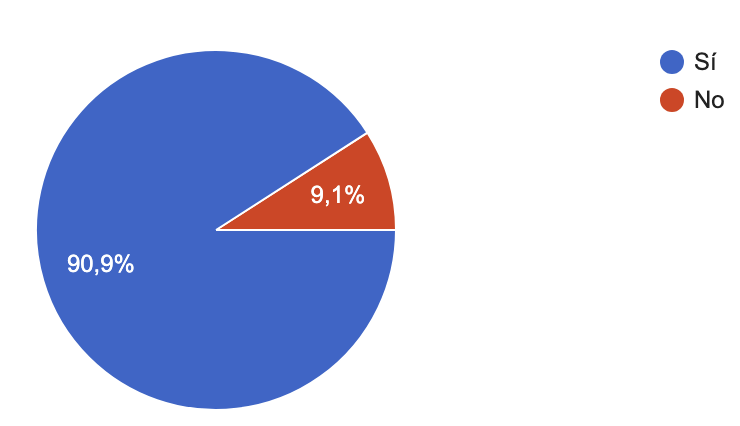
\includegraphics[width=0.5\linewidth]{Imagenes/Respuestas_Cuestionarios/r21.png}
    \caption{Uso de casos de prueba}
    \label{fig:uso_casos_prueba}
\end{figure}


\textbf{¿Con qué frecuencia compruebas si tus soluciones funcionan con casos de prueba propios?}
\begin{figure}[H]
    \centering
    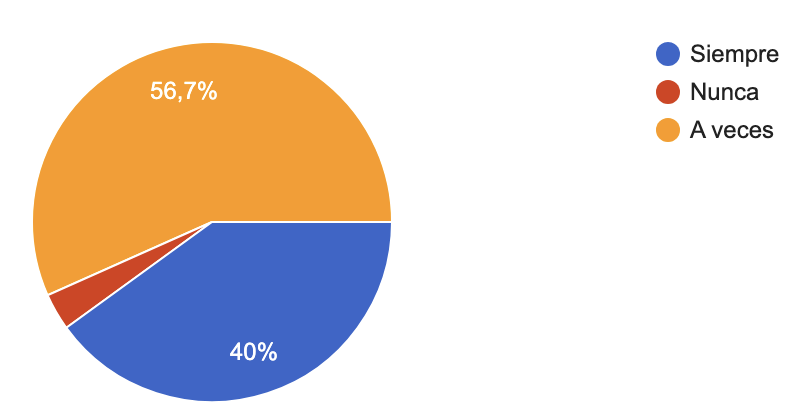
\includegraphics[width=0.5\linewidth]{Imagenes/Respuestas_Cuestionarios/r22.png}
    \caption{Uso de casos de prueba propios}
    \label{fig:uso_casos_prueba_propios}
\end{figure}

\textbf{Cuando intentas comprobar tus soluciones, ¿cómo generas tus casos de prueba?}
\begin{figure}[H]
    \centering
    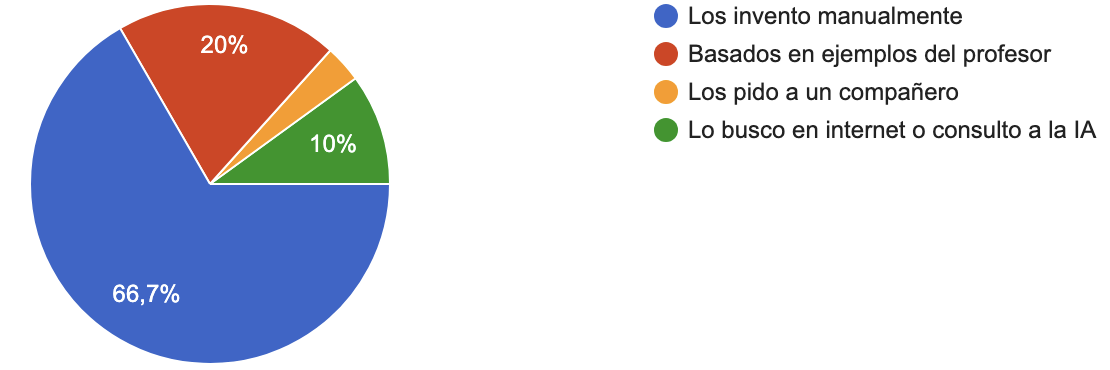
\includegraphics[width=0.7\linewidth]{Imagenes/Respuestas_Cuestionarios/r23.png}
    \caption{Métodos de generación de casos de prueba}
    \label{fig:métodos_generación_casos}
\end{figure}

\textbf{¿Te resulta complicado plantear tus propios casos de prueba?}
\begin{figure}[H]
    \centering
    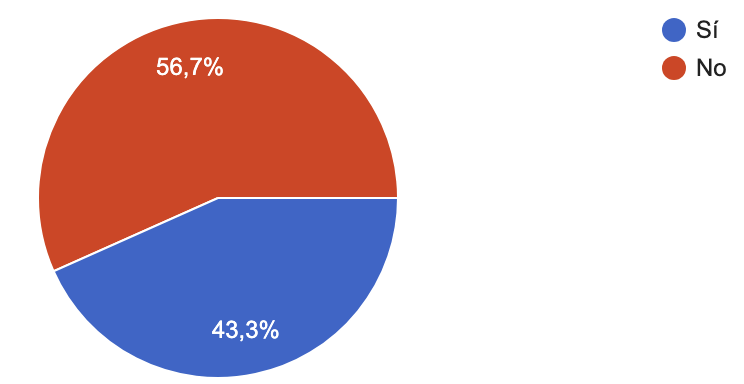
\includegraphics[width=0.5\linewidth]{Imagenes/Respuestas_Cuestionarios/r24.png}
    \caption{Dificultad generación casos de prueba propios}
    \label{fig:dificultad_generación_casos}
\end{figure}

\textbf{¿Cómo de útil te resulta una herramienta que genere contraejemplos mínimos basados en tu código?}
\begin{figure}[H]
    \centering
    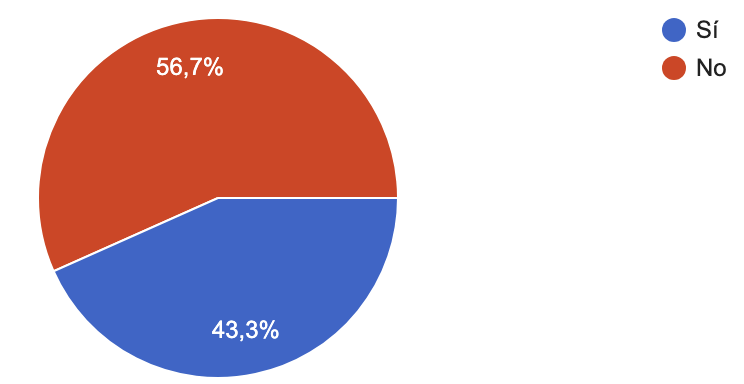
\includegraphics[width=0.5\linewidth]{Imagenes/Respuestas_Cuestionarios/r24.png}
    \caption{Dificultad generación casos de prueba propios}
    \label{fig:utilidad_herramienta_contraejemplos}
\end{figure}